\documentclass[11pt]{article}

\usepackage[margin=0.9in]{geometry}
\usepackage[T1]{fontenc}
\usepackage{lmodern}
\usepackage{microtype}
\usepackage{graphicx}
\usepackage{booktabs}
\usepackage{array}
\usepackage{longtable}
\usepackage{float}
\usepackage[hidelinks]{hyperref}

\setlength{\parindent}{0pt}
\setlength{\parskip}{6pt}
\renewcommand{\arraystretch}{1.12}

\title{IFEval Factor Interpretation Under a Product-Mixture Probit Factor Model}
\author{}
\date{Threshold $2/3$; full-data refit}

\begin{document}
\maketitle

\section{Fitted Model}

This note summarizes the full-data IFEval fit at threshold $2/3$, where an
item is scored as correct when the OpenEval strict-instruction score is at
least $2/3$.  The fitted model is the sparse product-mixture probit factor
model with
\[
  H=5,\qquad G=(3,3,2,3,3),\qquad \lambda_{\ell_1}=4.
\]
The binary response matrix contains 122 models and 538 nonconstant IFEval
items.  The converged full-data refit used sampled probit augmentation,
14 pretraining iterations, and 11 MAP refinement iterations.  All marginal
mixtures converged in the selected refinement iteration.  The fitted binary
log likelihood per observed response was $-0.246$.

Each factor coordinate is standardized by the fitted product-mixture scale
convention.  Larger positive scores therefore mean stronger performance on
items with positive loadings on that factor, after accounting for the other
coordinates and item intercepts.

\section{Loading Structure}

Figure~\ref{fig:lambda} shows the sparse loading matrix after sorting items by
their largest absolute loading.  The first factor is broad: most items have
their largest loading on F1.  The remaining factors carve out more local modes
of instruction-following difficulty.  The item counts by primary loading are:
F1 = 391, F2 = 65, F3 = 35, F4 = 34, and F5 = 13.

\begin{figure}[H]
\centering
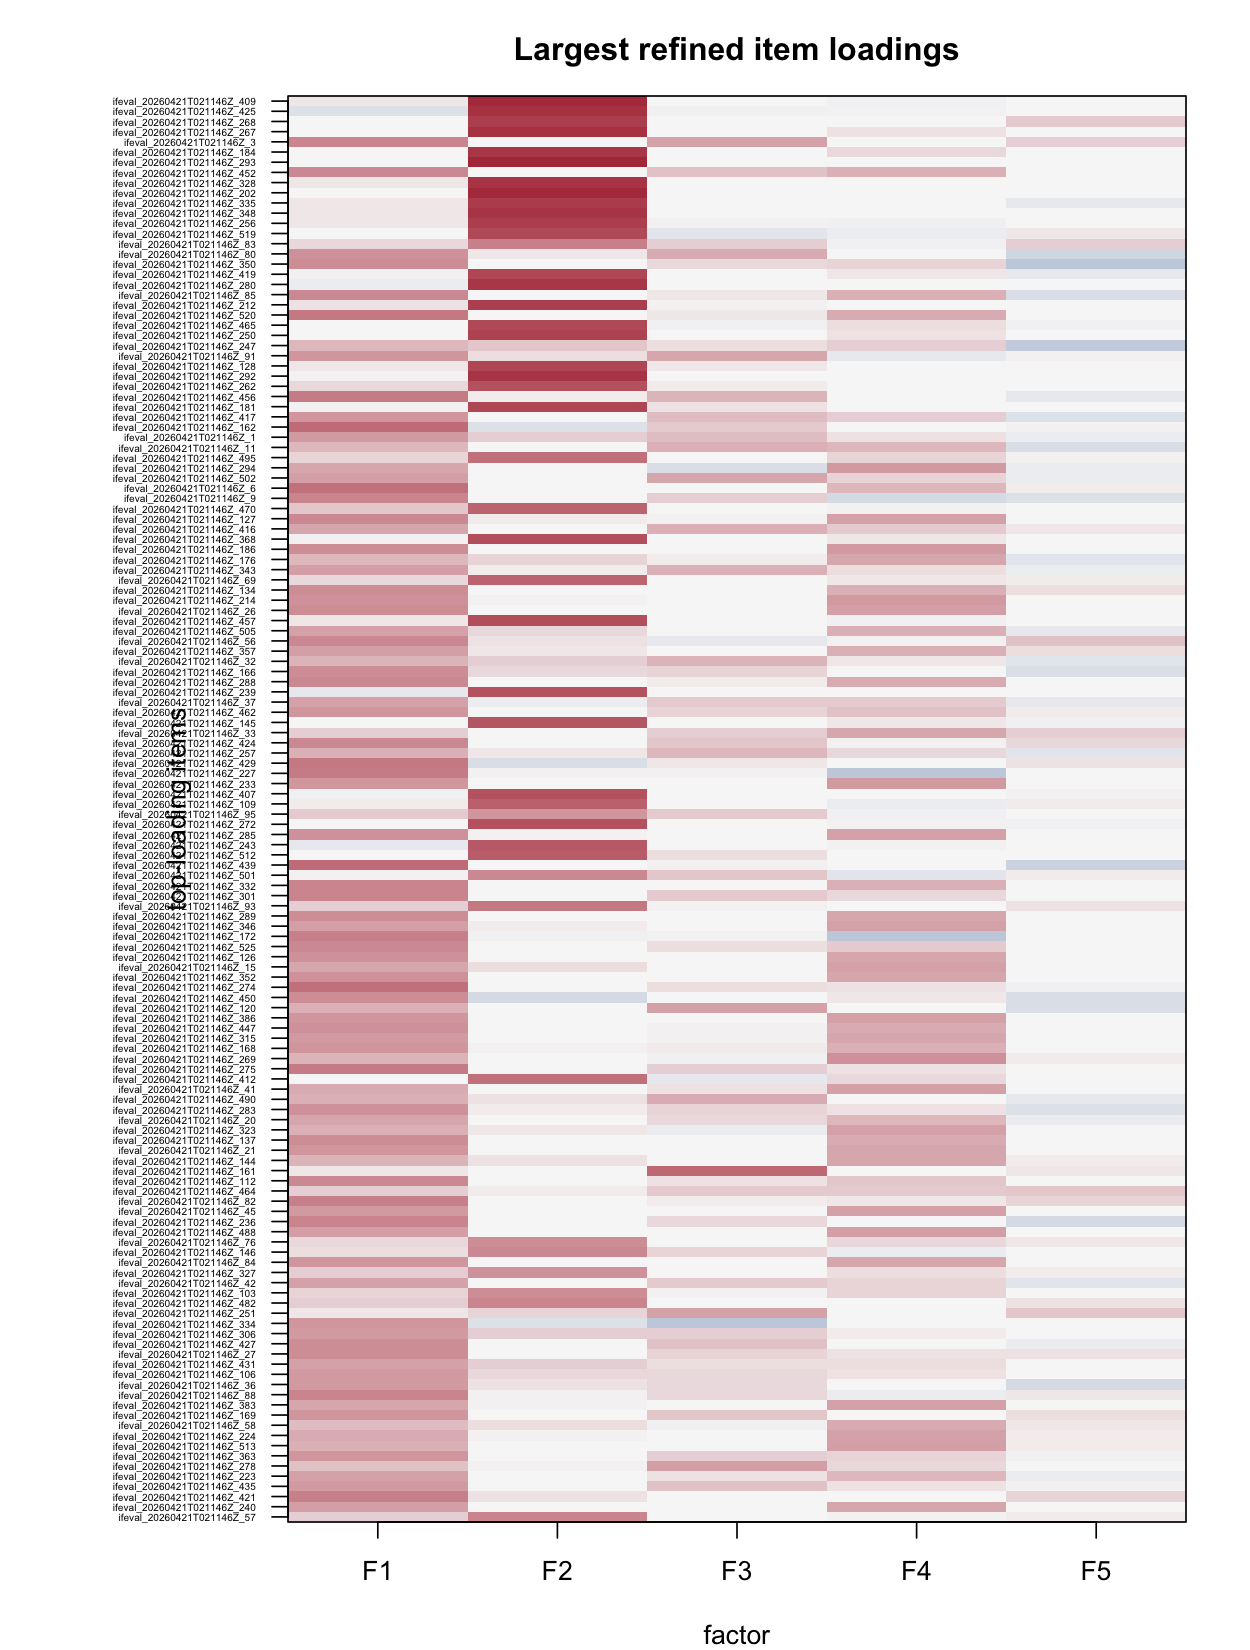
\includegraphics[width=0.92\linewidth]{top_item_loading_heatmap.png}
\caption{Estimated sparse loading matrix for the selected H=5 IFEval fit.
Rows are items, columns are factors, and rows are grouped by the factor with
largest absolute loading.}
\label{fig:lambda}
\end{figure}

\section{Factor Interpretation}

The factors are best read as overlapping psychometric modes rather than as the
25 raw IFEval instruction categories.  The model compresses those instruction
checks into five lower-dimensional axes:

\begin{center}
\begin{tabular}{p{0.08\linewidth}p{0.25\linewidth}p{0.57\linewidth}}
\toprule
Factor & Label & Interpretation \\
\midrule
F1 & Compositional response control &
Broad ability to satisfy multi-part prompts, repeated-prompt requirements,
sectioning, highlighting, paragraph structure, and several constraints at once. \\
F2 & Case and language mode control &
Ability to stay in a required surface mode, especially all-lowercase,
all-uppercase, and specified response language. \\
F3 & Lexical micro-control &
Fine token-level and count-based control: forbidden letters or words, letter
frequency, sentence counts, and unusually precise lexical inhibition. \\
F4 & Boundary and envelope formatting &
Formatting wrappers and response boundaries, including JSON, quotation marks,
and explicit ending constraints. \\
F5 & Length and count discipline &
Short-response length control, word limits, sentence limits, and count-based
keyword requirements. \\
\bottomrule
\end{tabular}
\end{center}

The instruction enrichment plots in Figure~\ref{fig:instr} support this
interpretation.  F2 is highly enriched for case and language instructions; F3
for letter-frequency and exact lexical/count constraints; F4 for JSON and
start/end wrappers; and F5 for compact length-control items.

\begin{figure}[H]
\centering
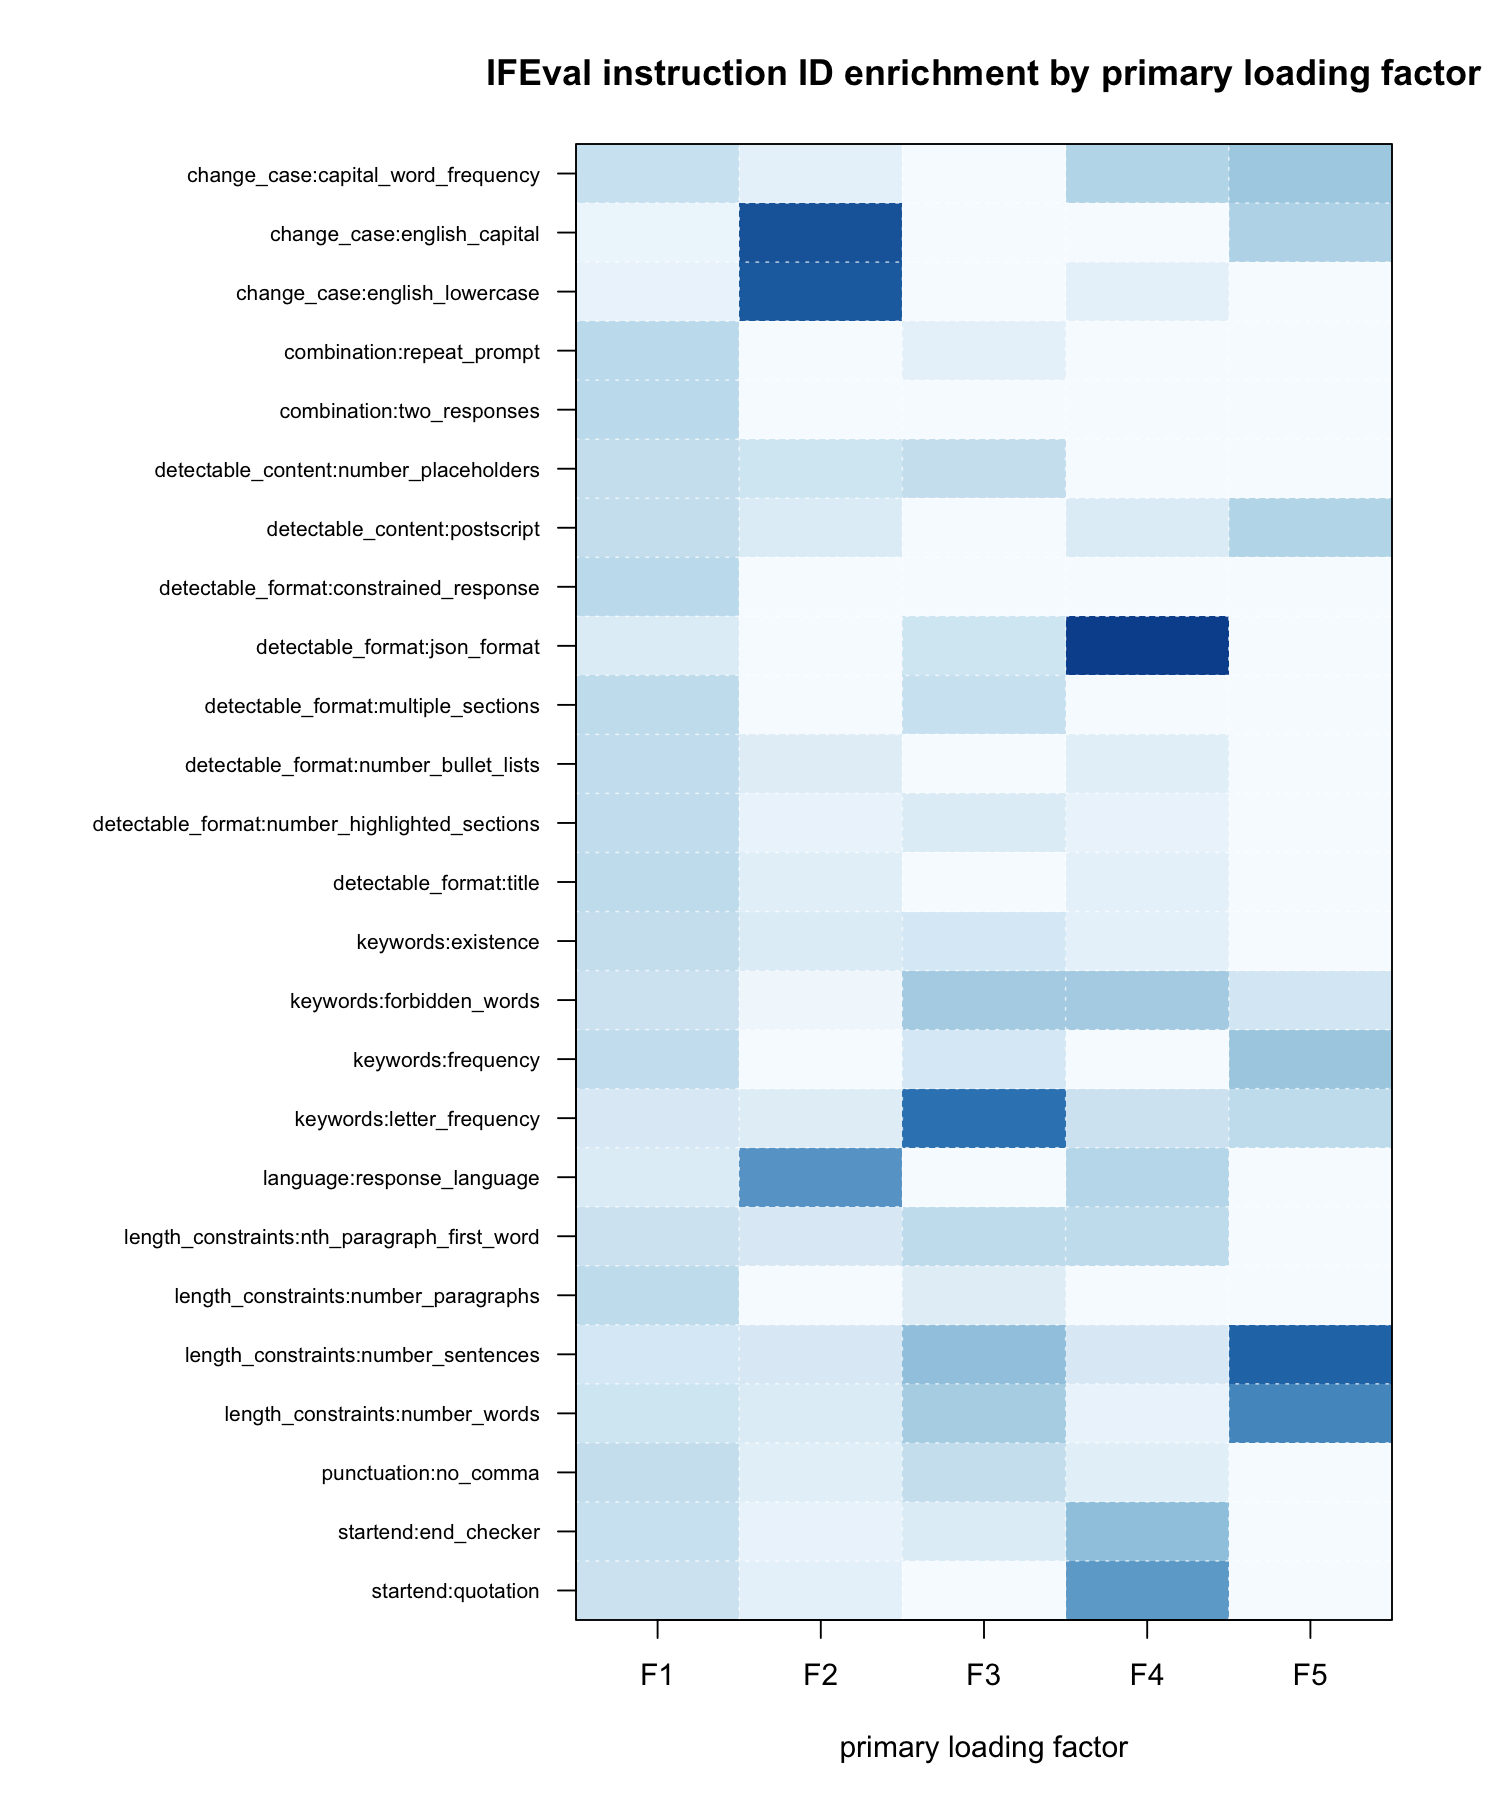
\includegraphics[width=0.98\linewidth]{instruction_id_lift.png}
\caption{Instruction-ID enrichment by primary factor.  Darker cells indicate
larger lift relative to the overall frequency of that instruction.}
\label{fig:instr}
\end{figure}

\begin{figure}[H]
\centering
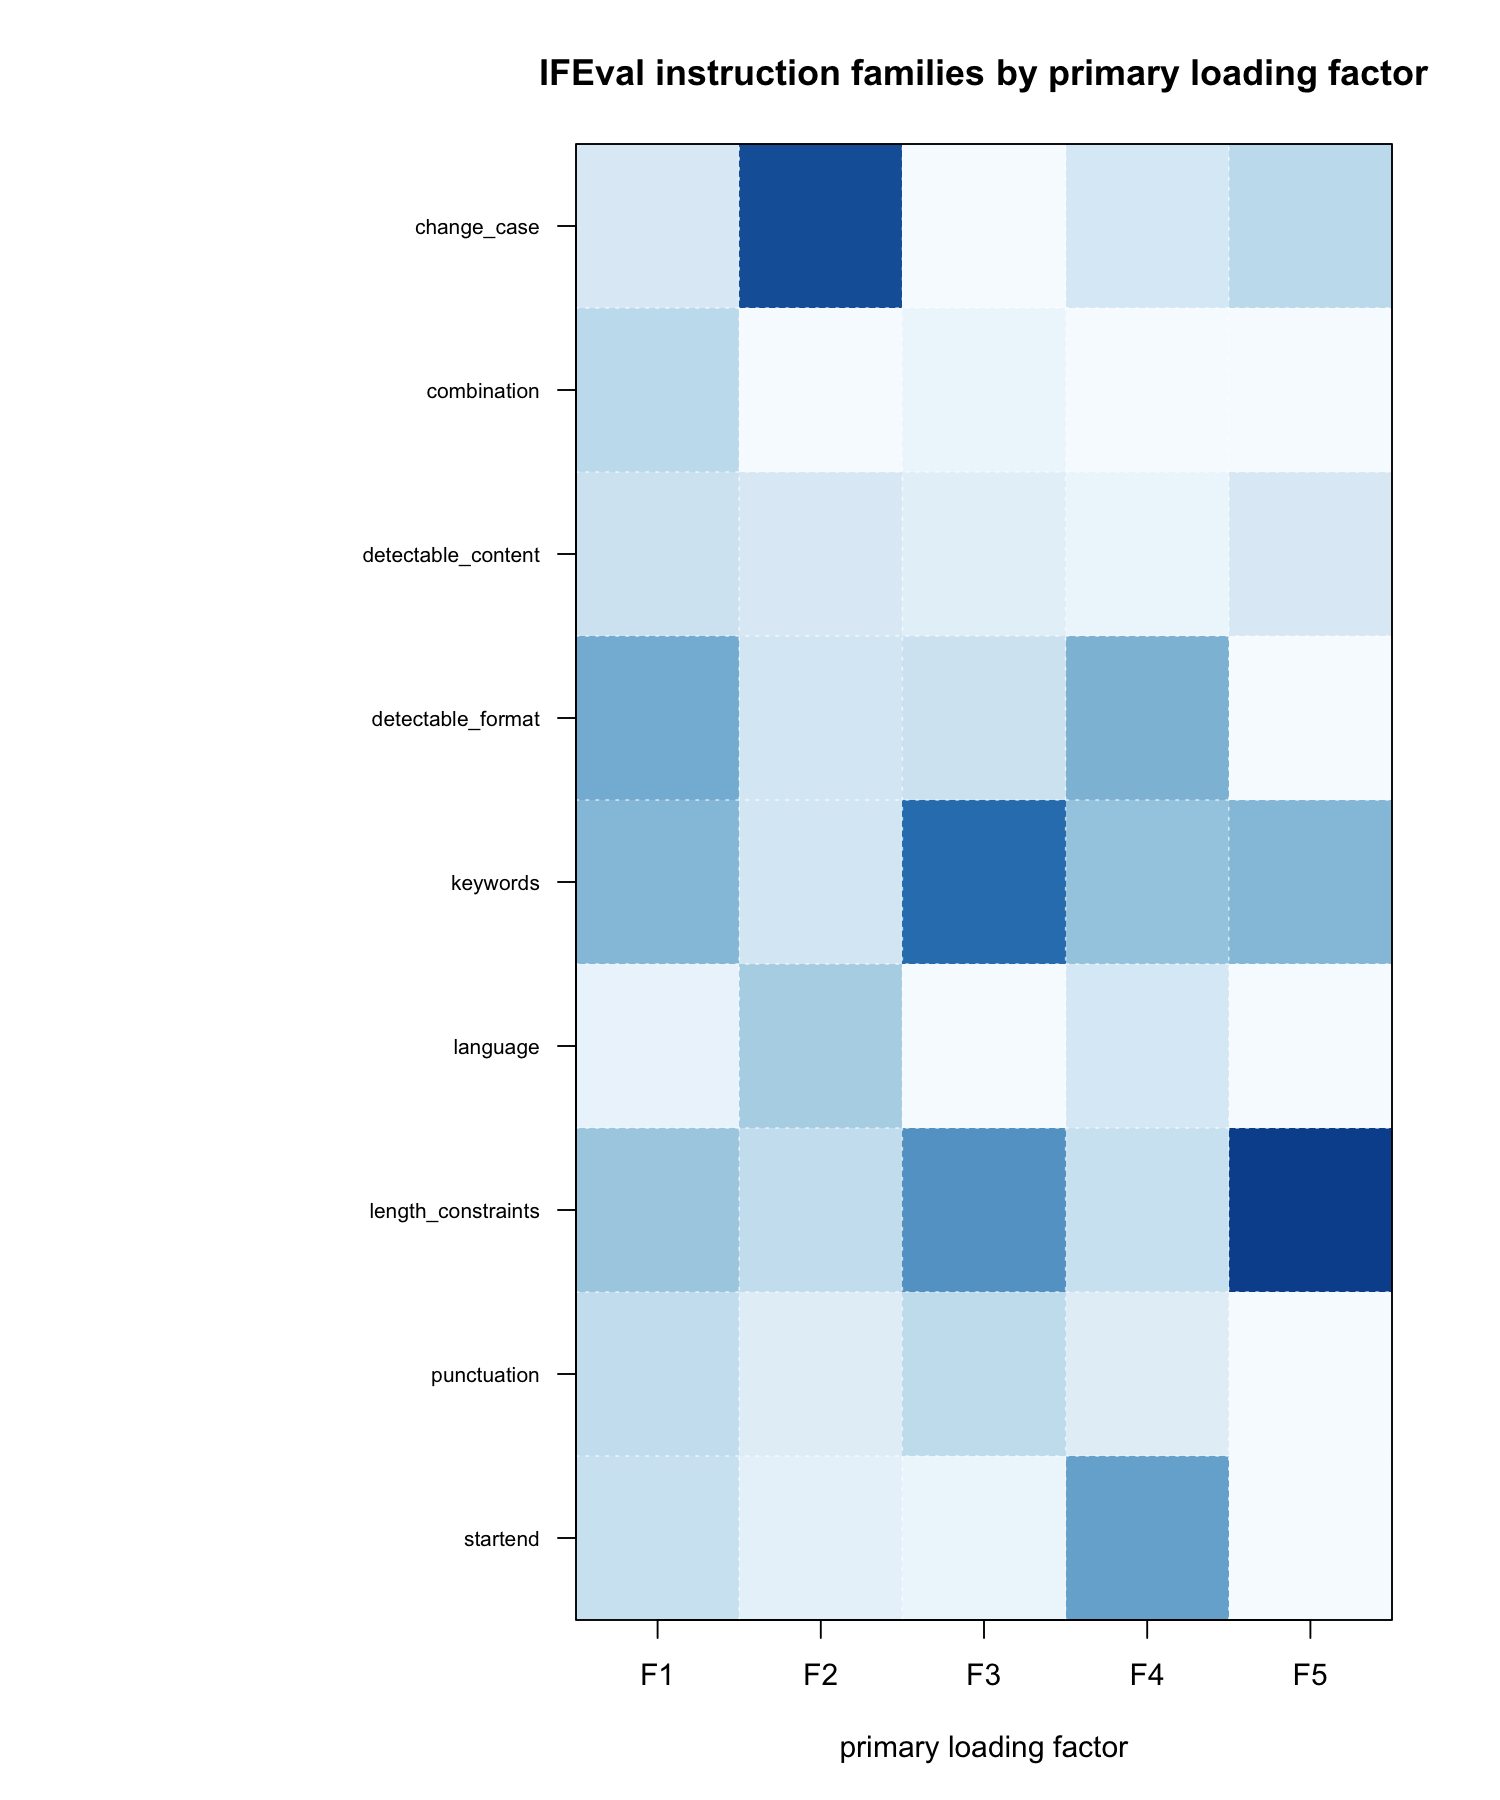
\includegraphics[width=0.86\linewidth]{instruction_family_proportion.png}
\caption{Instruction-family proportions within each primary factor group.}
\label{fig:families}
\end{figure}

\section{Strong Solo-Loading Items}

Table~\ref{tab:solo} gives examples whose primary loading is large and whose
second-largest absolute loading is comparatively small.  These are clean
representatives of each factor, although the factor labels should also be read
with the enrichment plots above.

\begin{longtable}{p{0.06\linewidth}p{0.10\linewidth}p{0.10\linewidth}p{0.66\linewidth}}
\caption{Strong mostly solo-loading item examples.  Accuracy is empirical
accuracy at the $2/3$ threshold.}\label{tab:solo}\\
\toprule
Factor & Item & Loading & Prompt excerpt \\
\midrule
\endfirsthead
\toprule
Factor & Item & Loading & Prompt excerpt \\
\midrule
\endhead
F1 & \texttt{\detokenize{...274}} & 1.779 &
Give two different responses to ``Is it ethical to hunt and eat invasive
species?'', separated by six asterisks and without using any commas. \\
F1 & \texttt{\detokenize{...242}} & 1.759 &
First repeat the request word for word, then give the answer; include a title
wrapped in double angular brackets. \\
F2 & \texttt{\detokenize{...293}} & 3.032 &
Create a product description for a product that helps stop snoring.  Use all
lowercase letters. \\
F2 & \texttt{\detokenize{...409}} & 2.969 &
Explain the difference between two-stroke and four-stroke motors; the entire
response must be in English and contain only lowercase letters. \\
F3 & \texttt{\detokenize{...161}} & 1.895 &
Continue and expand a scene description using at least 60 sentences but fewer
than 600 words. \\
F3 & \texttt{\detokenize{...277}} & 1.677 &
Write a rubric as a poem, with the letter ``w'' appearing fewer than two times. \\
F4 & \texttt{\detokenize{...50}} & 0.562 &
Write a haiku about rushing to work using only Marathi, with no other language
allowed. \\
F4 & \texttt{\detokenize{...217}} & 0.400 &
Rewrite a research-paper summary in APA format while avoiding specified words. \\
F5 & \texttt{\detokenize{...75}} & 0.522 &
Write a funny song with fewer than 10 sentences for a playground proposal. \\
F5 & \texttt{\detokenize{...232}} & 0.470 &
Write a template with fewer than seven sentences for calculating an array
offset. \\
\bottomrule
\end{longtable}

\section{Cross-Loading Items}

Cross-loading items are especially useful because they show why the factors are
not simply a relabeling of the raw instruction IDs.  A prompt can require a
general compositional skill plus one local control skill, or two local skills
at once.

\begin{longtable}{p{0.10\linewidth}p{0.18\linewidth}p{0.18\linewidth}p{0.46\linewidth}}
\caption{Representative cross-loading item examples.}\label{tab:cross}\\
\toprule
Pair & Primary loading & Secondary loading & Prompt excerpt \\
\midrule
\endfirsthead
\toprule
Pair & Primary loading & Secondary loading & Prompt excerpt \\
\midrule
\endhead
F1/F4 & F1 = 1.317 & F4 = 1.230 &
Give an opinion on Kareena Kapoor and wrap the entire response in double
quotation marks. \\
F1/F3 & F1 = 1.497 & F3 = 1.091 &
Write a resignation email, repeat the request verbatim first, and obey
additional lexical restrictions. \\
F1/F5 & F1 = 1.132 & F5 = -0.785 &
Give advice about a dime in the style of a U.S. president and make the response
at least 600 words. \\
F3/F4 & F3 = 0.873 & F4 = 0.765 &
Create a product advertisement, with the entire output in JSON format. \\
F2/F5 & F2 = 1.176 & F5 = 0.686 &
Explain the difference between a levee and an embankment, responding only in
Korean. \\
F1/F2 & F1 = 0.888 & F2 = 0.663 &
Write a long funny sales pitch while satisfying a word-length target and other
surface-form constraints. \\
F3/F5 & F3 = 1.213 & F5 = -0.618 &
Write an investor-facing essay about the history of the Internet with at least
50 sentences. \\
F2/F3 & F2 = 1.418 & F3 = 0.580 &
Write a professional but weird cover letter with a strict letter-frequency
constraint. \\
F2/F4 & F2 = 1.772 & F4 = 0.376 &
Write an all-capital, coach-like article with no lowercase letters. \\
\bottomrule
\end{longtable}

\section{Marginal Mixtures and LLM Profiles}

Figure~\ref{fig:marginals} shows the fitted one-dimensional mixtures for the
five factor scores.  The fitted groups are ordered by their means within each
coordinate, so cluster labels are coordinate-specific.  For example, a high
cluster on F1 is not the same population subset as a high cluster on F3.

\begin{figure}[H]
\centering
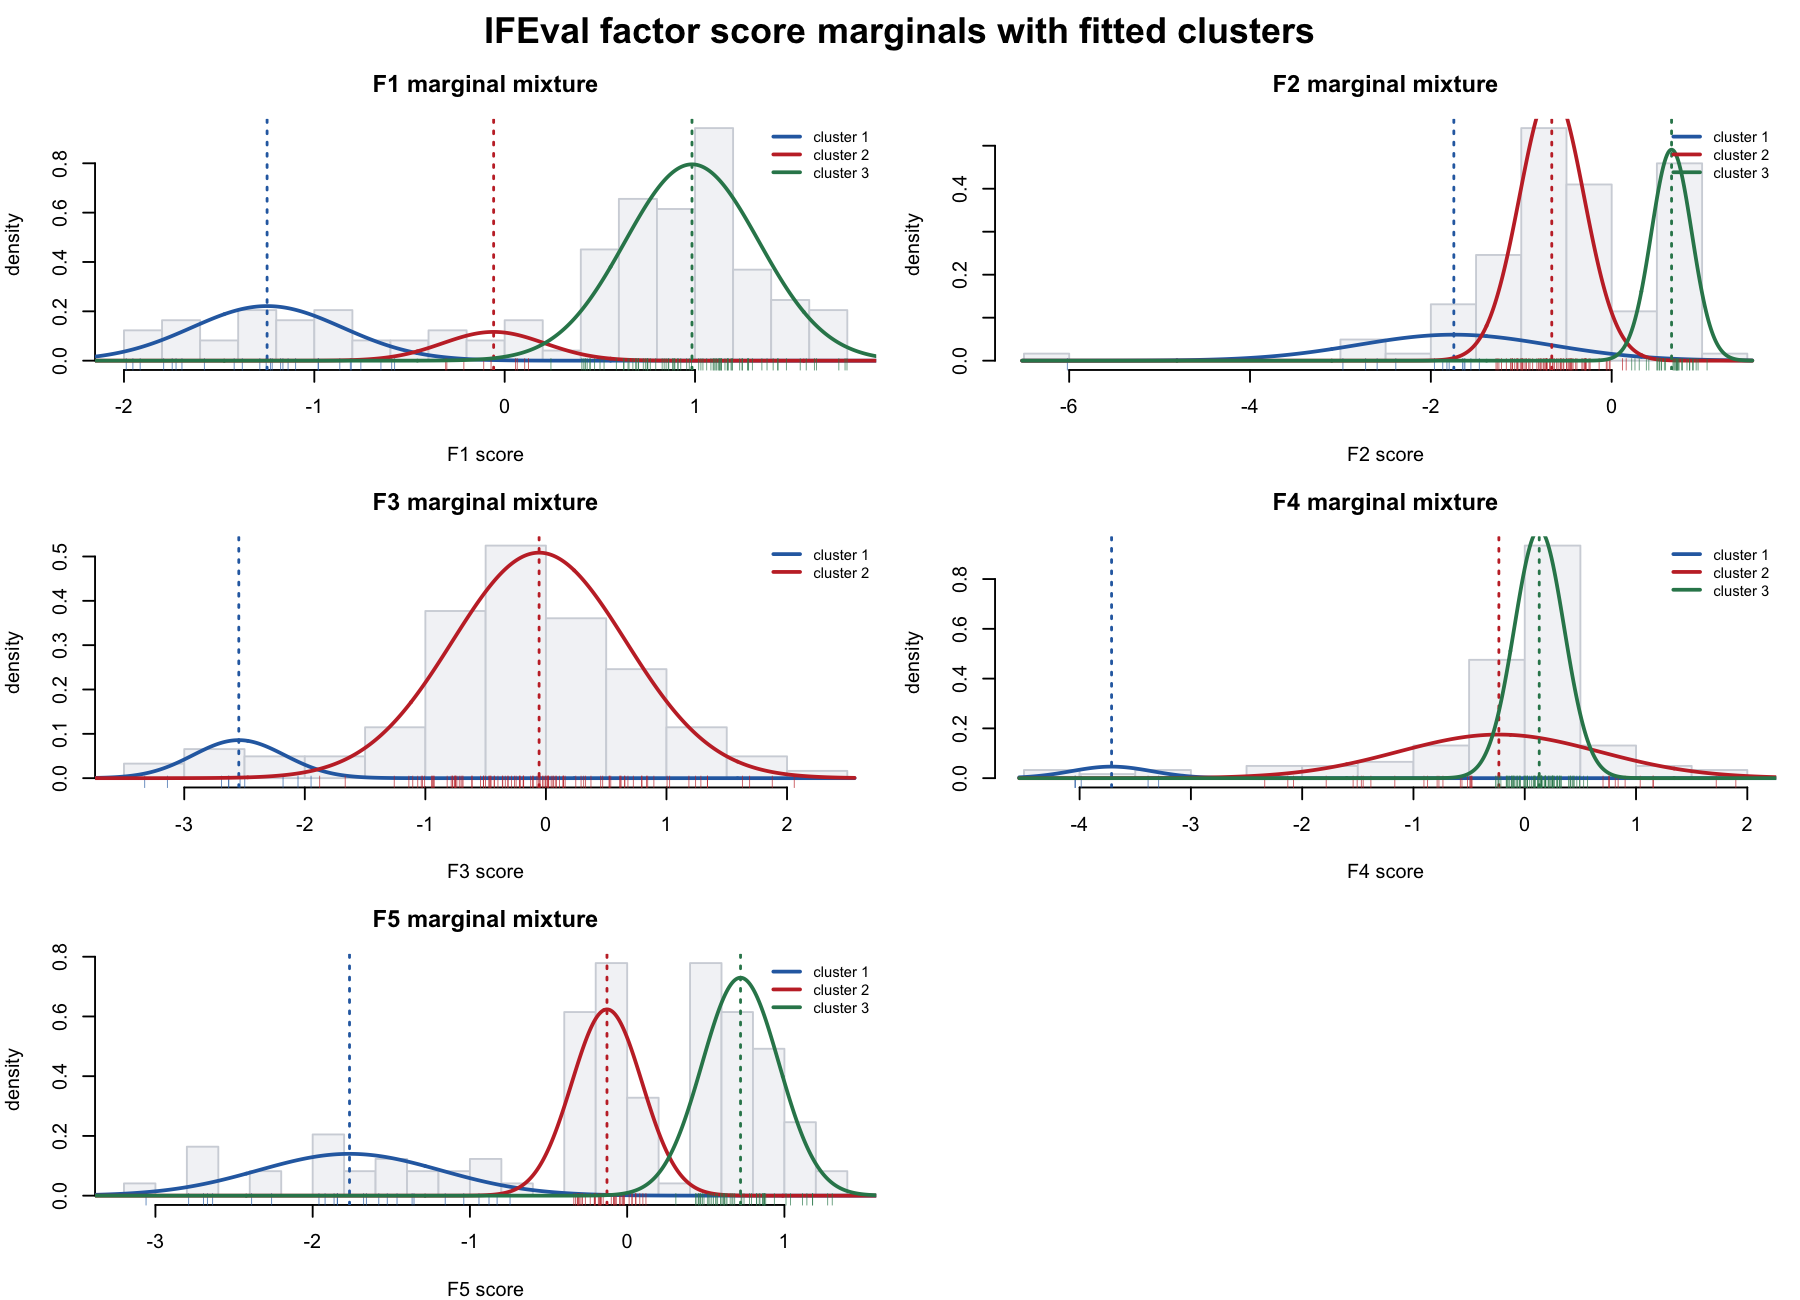
\includegraphics[width=0.98\linewidth]{factor_marginal_mixtures.png}
\caption{Estimated marginal distributions of the five factor coordinates with
fitted mixture components overlaid.}
\label{fig:marginals}
\end{figure}

The joint profiles give a compact description of model behavior.  The strongest
overall models, such as \texttt{gpt-5.4-pro-2026-03-05},
\texttt{gpt-5.2-pro-2025-12-11}, and \texttt{grok-4-0709}, tend to be high on
F1 and not weak on the local factors.  Some models have uneven profiles:
\texttt{gpt-5-2025-08-07} is very high on F3 but low on F2, suggesting strong
lexical/count control but weaker case/language mode control in this fitted
coordinate system.  Smaller or older models often have low F1 and weak local
coordinates; this predicts failures on prompts that combine several constraints
with exact formatting, casing, or count requirements.

This is the main psychometric value of the model: it does not merely rank
models by average IFEval accuracy.  It separates broad compositional control
from local failure modes, and it gives each LLM a joint ability profile that can
be linked back to concrete prompt types.

\section{Takeaway}

The H=5, $G=(3,3,2,3,3)$ fit suggests that IFEval is much lower-dimensional
than its 25 instruction IDs, but not one-dimensional.  F1 captures broad
multi-constraint response control, while F2--F5 isolate specific surface-form,
lexical, boundary-formatting, and length/count abilities.  Cross-loading items
are not nuisances: they are the items that reveal how these skills interact in
real instruction-following prompts.

\end{document}
